\documentclass[acmtog]{acmart}
\usepackage{graphicx}
\usepackage{subfigure}
\usepackage{natbib}
\usepackage{listings}
\usepackage{bm}

\definecolor{blve}{rgb}{0.3372549 , 0.61176471, 0.83921569}
\definecolor{gr33n}{rgb}{0.29019608, 0.7372549, 0.64705882}
\makeatletter
\lst@InstallKeywords k{class}{classstyle}\slshape{classstyle}{}ld
\makeatother
\lstset{language=C++,
	basicstyle=\ttfamily,
	keywordstyle=\color{blve}\ttfamily,
	stringstyle=\color{red}\ttfamily,
	commentstyle=\color{magenta}\ttfamily,
	morecomment=[l][\color{magenta}]{\#},
	classstyle = \bfseries\color{gr33n}, 
	breaklines=true, 
	tabsize=2
}
\lstset{basicstyle=\ttfamily}

% Title portion
\title{Assignment 4:\\ {Global Illumination}}

\author{Name:\quad Yang Hongdi  \\ student number:\ 2019533234
\\email:\quad yanghd@shanghaitech.edu.cn}

% Document starts
\begin{document}
\maketitle

\vspace*{2 ex}

\section{Introduction}
In this project, ray tracing with direct and indirect lighting is performed using Monte-Carlo integration. BVH-tree is used for acceleration.
\section{Implementation Details}
\subsection{Acceleration : BVH}
	In this project, to accelerate ray-triangle intersection, BVH is used. When building BVH, SAH is used for best space division.\\
	First, we sort the triangles by the coordinate of its center, then we save the result of all possible space division by the triangles. Then we compute the time cost of each space division
	by using the formula $$c(A,B) = t_{trav} + p_A\sum_{i=1}^{N_A}t_{isect}(ai) + p_B\sum_{i=1}^{N_B}t_{isect}(b_i)$$
	where we set $p_A,p_B$ equal to the surface area of the AABB, $t_isect = 1, t_{trav} = 0$, and we choose the space division with the minimum time cost as the 
	best space division. We repeat this for all three axis and then choose the best axis to split the space.\\
	Now we get the best spcae division, we store the left AABB and the right AABB with their triangles, then we continue to split the space recursively.
	Until we just have only a few triangles or enough recursion depth, the we store the node as leaf node and store the triangles.
	\begin{lstlisting}
		// recursively build left and right
    leftChild = new KdTreeNode(leftTriangles, leftSpace, depth + 1);
    rightChild = new KdTreeNode(rightTriangles, rightSpace, depth + 1);
	\end{lstlisting} 
	For intersection test, we just first check whether the ray hit the bouding box, if it does not, end checking directly and return false.
	\begin{lstlisting}
		if (!this->box.rayIntersection(ray, tIn, tOut)) return false; // not intersect with bounding box, return false directly.
	\end{lstlisting}
	If it hits the bouding box, we then recursively check whether it hits the left and right child bouding box. When the hit the light hit the leaf node, we just
	violently check if it hits the triangles inside the bouding box. Finally, we return true with the nearest triangle that has been hit.
\subsection{Path tracing with Monte-Carlo integration}
In this project, path tracing with Monte-Carlo integration is performed.
\subsubsection{Ideal Diffusion BRDF}
	\quad For ideal diffusion BRDF, we use cos-weighted sampling. We first sample uniformly on a disk.
	\begin{lstlisting}
		auto random_samples = unif(0.0, 1.0, 2);

	//sampling on a disk
	Float x1 = random_samples[0];
	Float y1 = random_samples[1];
	\end{lstlisting}
	Then we transform (x,y) to $(r,\theta_1)$, $$r = \sqrt{x_1}, \theta_1 = 2\pi y_1 $$
	then we project it onto the unit hemisphere. we need to transform $(r, \theta_1)$ to $(\theta, \phi)$(Note: $\theta$ is different from $\theta_1$)
	$$\sin\theta = r = \sqrt{x_1}, \phi = \theta_1 = 2\pi y_1 $$
	then we can compute $$ x = \sin\theta\cos\phi $$$$ y = \sin\theta\sin\phi $$$$ z = \cos\theta$$
	Last, we convert it from local coordinate to world coordinate using the normal.
	\begin{lstlisting}
		vec3 rotation_axis = vec3(0,0,1).cross(interact.normal);
	Eigen::AngleAxisf rotationVector(theta, rotation_axis);
	Eigen::Matrix3f rotation_matrix = rotationVector.toRotationMatrix();
	interact.wi = -(rotation_matrix * tmp_wi).normalized(); // from (0,0,1) system to world coordinate
	\end{lstlisting}
	Then we get the sampled incoming ray. And the pdf equal to $\frac{cos\theta}{\pi}$
\subsubsection{Ideal Specular BRDF}
	\quad For Ideal Specular BRDF, it is quite easy. We simply sample the reflect light, which should have a pdf of 1.
	The reflect direction can be computed by $$w_i = 2(w_o \cdot n)n - w_o$$
\subsubsection{Ideal Transmission BRDF}
	\quad For Ideal Transmission BRDF, similar as Ideal Specular, we sample the refraction light, which also have a pdf of 1.
	We use $$w_i = \frac{\eta_1}{\eta_2}w_o + (\frac{\eta_1}{\eta_2}\cos \theta_i - \sqrt{1 - \sin^2 \theta_t})n$$
	If we find that $\cos \theta_i < 0$, that means the ray is inside the object, we will then let $\cos \theta_{i_1} = -\cos \theta_{i}, n_1 = -n, \frac{\eta_{1_1}}{\eta_{2_1}} = \frac{\eta_2}{\eta_1}$ to compute the next ray.
\subsubsection{Glossy Specular}
	\quad For Glossy Specular, Disney principle BRDF is choosed to simulate Glossy surface BRDF. Multiple importance sampling is used.
	First, we calculate all angles as the graph shows.
	\begin{figure}[H]
		\centering
		
		\subfigure[Scene0]{
		\begin{minipage}[t]{0.45\linewidth}
		\centering
		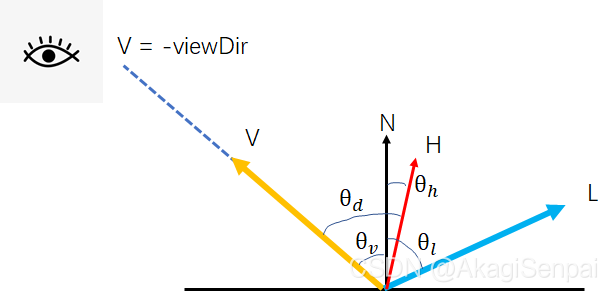
\includegraphics[width=1.5in]{images/angles.png}
		%\caption{original image}
		\end{minipage}%
		}
	\end{figure}
	We let $$spec = D(\theta_h)F(\theta_d)G(\theta_l,\theta_v)$$
	where $$D_{GTR}(\theta_h) = \frac{\alpha}{\pi}\frac{1}{(1 + (\alpha^2-1)\cos^2\theta_h)^2}$$ $$\alpha = roughness^2$$
	$$F(\theta_d) = 0.08 + (1- 0.08)(1-\cos \theta_d)^5$$
	$$G(v) = \frac{n \cdot v}{(n \cdot b) + \sqrt{\alpha^2 + (1-\alpha^2)(n \cdot v)^2}}$$
	And we use BRDF weighted sampling to sample the reflect ray. i.e
	$$pdf_h = D(\theta_h)\cos\theta_h, \ pdf_l = \frac{pdf_h}{4(l \cdot h)}$$
	we sample both the light and brdf, then combine them with multiple importance sampling.
	$$dirlight = \frac{pdf_{light}^2}{pdf_{light}^2 + pdf_{brdf}^2}L_{light} + \frac{pdf_{brdf}^2}{pdf_{light}^2 + pdf_{brdf}^2}L_{brdf}$$
	\subsubsection{Area light sampling}
	To sample on the rectangle area light is quit easy. we just uniformly sample a point on the rectangle area light.
	\begin{lstlisting}
		auto random_sample = unif(0.0, 1.0, 2);
    Float x1 = random_sample[0];
    Float z1 = random_sample[1];
    vec3 sample_position = position + ((x1 - 0.5) * areaSize[0] * vec3(1, 0, 0)) + ((z1 - 0.5) * areaSize[1] * vec3(0, 0, 1));//uniformly ramdom choose a point on arealight
	\end{lstlisting}
	and the pdf will be $\frac{1}{A}$.
	However, as $$L_o(x,w_o) = \int_{\Omega}L_i(p,w_i)f_r(p,w_i,w_o)(n\cdot w_i)dw_i$$
	we need to transform $dw_i$ to $d_A$. By the definition of solid angle, we have $dw = \frac{dA \cos\theta^{'}}{||x^{'} - x||^2}$, where 
	$\cos\theta^{'} = n_{light} \cdot w_i$, $x^{'}$ is our sampled position on light, $x$ is the intersection point. Then we have
	$$L_o(x,w_o) = \int_{\Omega}L_i(p,w_i)f_r(p,w_i,w_o)\frac{\cos\theta\cos\theta^{'}}{||x^{'} - x||^2}dA$$
	here is the code for computing solid angle.
	\begin{lstlisting}
	auto geom = geoms[0];
    Float cos_theta1 = abs(geom.get()->getNormal().dot(ref_it.wi));
    Float distance = (pos - ref_it.entryPoint).norm();
    return cos_theta1 / (distance * distance); // solid angle of the tiny surface
	\end{lstlisting}
	\subsubsection{Integrator based on Monte-Carlo Path Tracing}
	For each ray, we perform Monte-Carlo Path Tracing with following recursive procedure.
	\begin{lstlisting}
	shade(p, wo, depth)
		Check if depth > MAX_DEPTH return vec3(0,0,0)
		If hit light, check (n * wo) return light emission
		If hit object, sample the light at x1
		L_dir = L_i * f_r * cos_theta *cos_theta1/|x1-p|^2/pdf_light
		shoot another ray to compute indirect lighting
		Ray r(p, wi)
		If r hit anything at position q
		L_indir = shade(q, wi, depth + 1) * f_r * cos_theta/pdf
		return L_dir + L_indir
	\end{lstlisting}
	\section{Results}
	\begin{figure}[H]
		\centering
		
		\subfigure[Scene0]{
		\begin{minipage}[t]{0.45\linewidth}
		\centering
		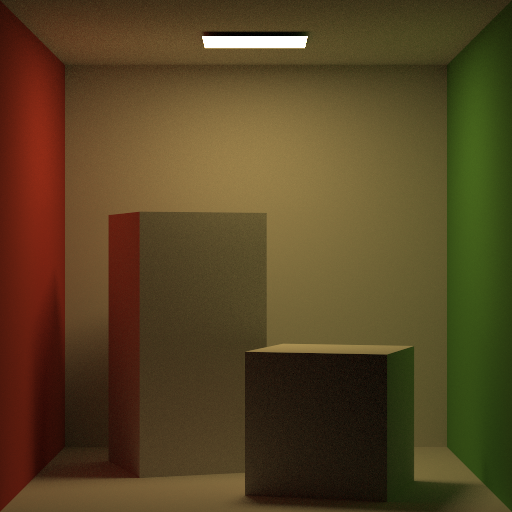
\includegraphics[width=1.5in]{images/output_256.png}
		%\caption{original image}
		\end{minipage}%
		}
		\subfigure[Scene1]{
		\begin{minipage}[t]{0.45\linewidth}
		\centering
		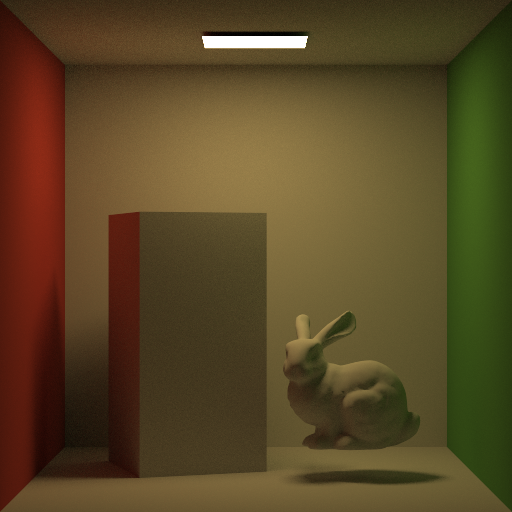
\includegraphics[width=1.5in]{images/output_bunny.png}
		%\caption{ground truth}
		\end{minipage}%
		}%
						
		\subfigure[Scene2]{
		\begin{minipage}[t]{0.45\linewidth}
		\centering
		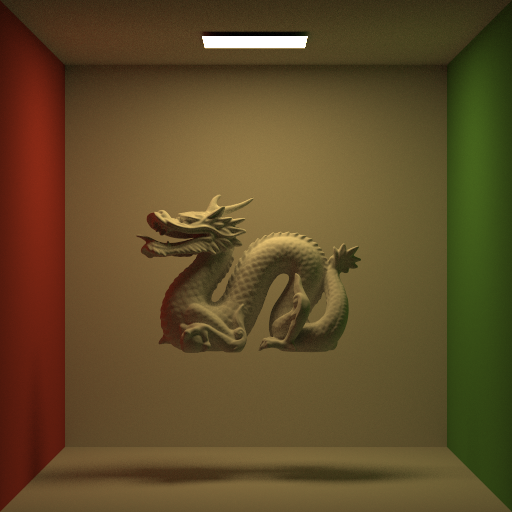
\includegraphics[width=1.5in]{images/output_dragon1.png}
		%\caption{depth prediction result}
		\end{minipage}
		}
		\subfigure[Scene3]{
		\begin{minipage}[t]{0.45\linewidth}
		\centering
		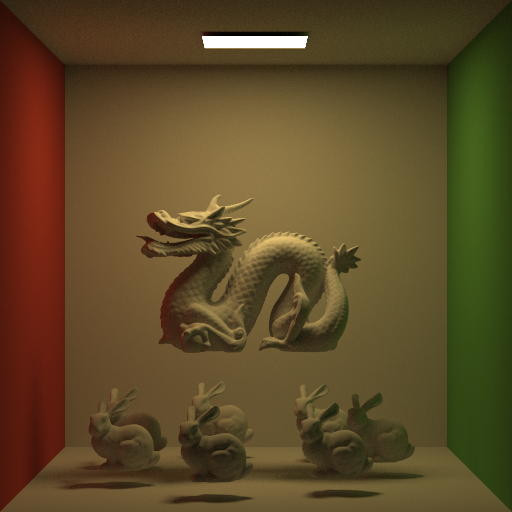
\includegraphics[width=1.5in]{images/output_dragon_bunny.png}
		%\caption{depth prediction result}
		\end{minipage}
		}
		\subfigure[Scene4]{
		\begin{minipage}[t]{0.45\linewidth}
		\centering
		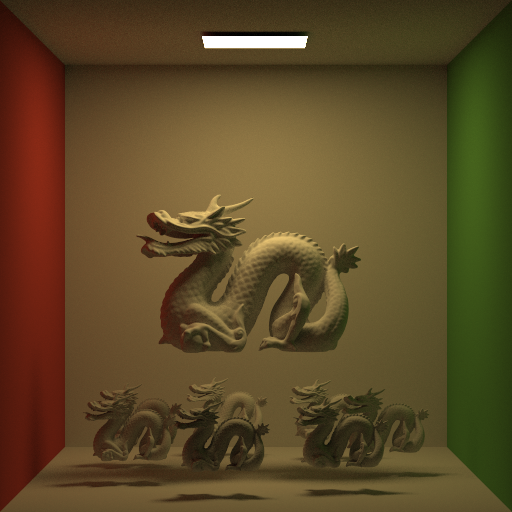
\includegraphics[width=1.5in]{images/output_all_dragon.png}
		%\caption{depth prediction result}
		\end{minipage}
		}
		\subfigure[Scene0spp512]{
		\begin{minipage}[t]{0.45\linewidth}
		\centering
		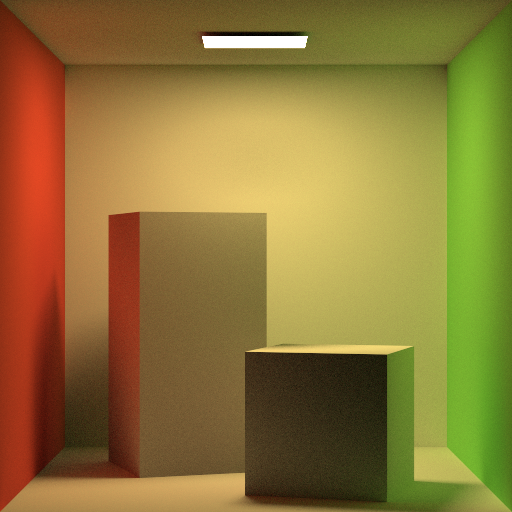
\includegraphics[width=1.5in]{images/output_birghter_512.png}
		%\caption{depth prediction result}
		\end{minipage}
		}
		\subfigure[Scene1spp512]{
		\begin{minipage}[t]{0.45\linewidth}
		\centering
		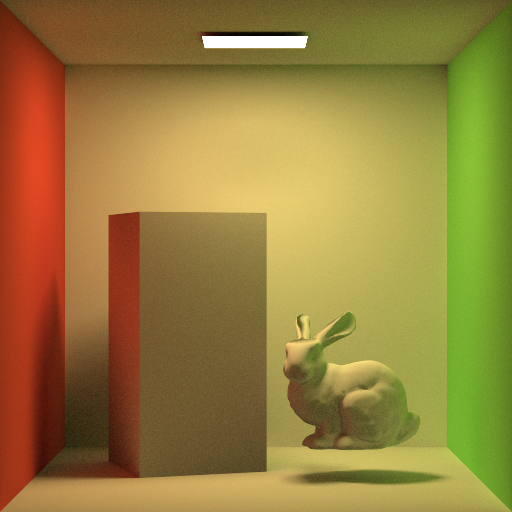
\includegraphics[width=1.5in]{images/output_bunny_512.png}
		%\caption{depth prediction result}
		\end{minipage}
		}
		\subfigure[Scene1specular]{
		\begin{minipage}[t]{0.45\linewidth}
		\centering
		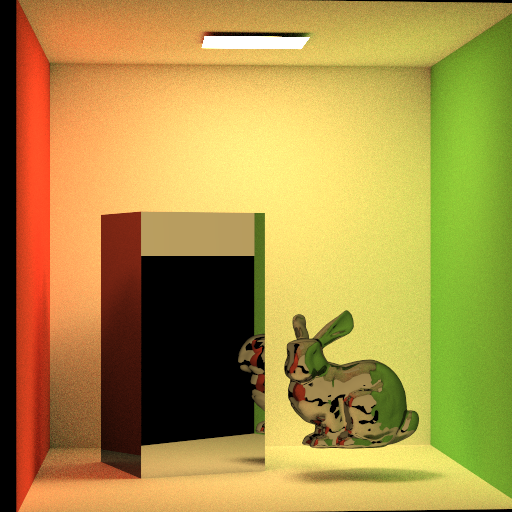
\includegraphics[width=1.5in]{images/output_spec.png}
		%\caption{depth prediction result}
		\end{minipage}
		}
		\subfigure[Scene2Transmission]{
		\begin{minipage}[t]{0.45\linewidth}
		\centering
		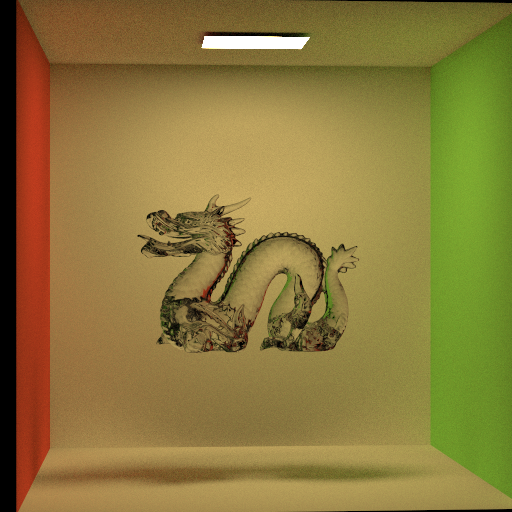
\includegraphics[width=1.5in]{images/output_dragon_transmission_depth6.png}
		%\caption{depth prediction result}
		\end{minipage}
		}
		\subfigure[Scene1Glossy]{
		\begin{minipage}[t]{0.45\linewidth}
		\centering
		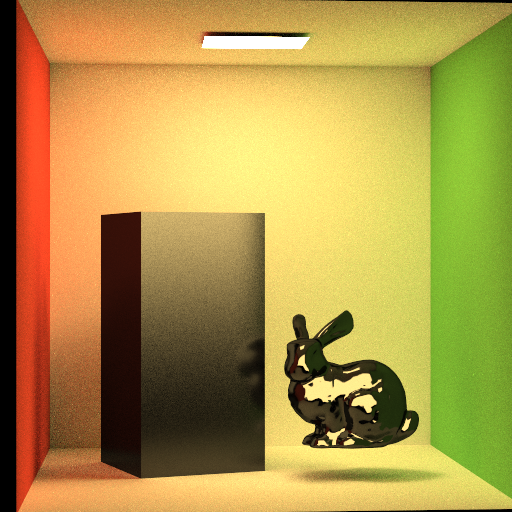
\includegraphics[width=1.5in]{images/output_glossy_box0.2_bunny0.1.png}
		%\caption{depth prediction result}
		\end{minipage}
		}
		\end{figure}
\end{document}
